\documentclass[a4paper,12pt]{article}
\usepackage{graphicx} 
\usepackage{amsmath}   
\usepackage{hyperref} 
\usepackage{geometry}  
\usepackage[ngerman]{babel}
\geometry{top=2.5cm,bottom=2.5cm,left=2.5cm,right=2.5cm}

\begin{document}
	
\begin{titlepage}
	\begin{flushleft}
		
\includegraphics[width=4cm]{../../data/Dokumentation_ScreenShots/logo.png} \\[0.5cm]
		Fakultät 10, Informatik
	\end{flushleft}
	
	\vspace{2.5cm}
	
	\begin{center}
		{\Large Dokumentation des Billard Spiels} \\[0.7cm]
		{\large WASP Projekt} \\[1.2cm]
		
		Studiengang: Allgemeine Informatik \\[1.5cm]
		
		Autoren: \\[0.3cm]
		Dimitrij Pivovar, Ivan Kurilin
	\end{center}
	
	\vfill
	\begin{flushleft}
		Betreut von: \\
		Prof. Dr. Wolfgang Konen \\
		Dr. rer. nat., Dipl.-Phys.
	\end{flushleft}
	
	\vspace{0.8cm}
	
	\begin{flushleft}
		Köln, \today
	\end{flushleft}
\end{titlepage}
	

	
	\newpage


	\tableofcontents
	
	\newpage
	\section{Einleitung}
	In diesem Projekt haben wir eine Billard Simulation entwickelt, die sowohl eine realistische grafische Darstellung als auch physikalische Interaktionen der Kugeln berücksichtigt. Ziel war es, eine funktionierende Simulation zu erstellen, die die Bewegungen und Kollisionen der Kugeln realistisch darstellt. Das Projekt stellt eine interessante Herausforderung im Bereich der Spieleentwicklung dar, da es sowohl unterhaltsame als auch physikalische Simulationen kombiniert. Es bietet wertvolle Einblicke in die Entwicklung realistischer Spiele und die Anwendung von Kollisionserkennung und -berechnungen, die auch in anderen Bereichen der Spieleentwicklung relevant sind.
	
	Diese Dokumentation bietet einen Überblick darüber, wie das Programm funktioniert, wie wir das System evaluiert haben, sowie eine Beschreibung der auftretenden Artefakte und Herausforderungen.
	
	\section{Grundlagen}
	\subsection{Spielregeln}
	Das Spiel basiert auf der 8 Ball Variante des Billards. Zwei Spieler treten gegeneinander an. Zu Beginn wird eine der beiden Gruppen von Kugeln zugewiesen: entweder die "vollen" oder die "halben" Kugeln. Ziel des Spiels ist es, alle Kugeln der eigenen Gruppe korrekt in die Taschen zu versenken und zuletzt die schwarze 8 Ball korrekt zu versenken, um zu gewinnen.
	
	Der Spieler, der seine Kugeln zuerst versenkt, muss danach die 8 Ball versenken, um das Spiel zu gewinnen. Versenkt der Spieler die 8 Ball vorzeitig oder auf unkorrekte Weise, verliert er das Spiel.
	\subsection{Punktesystem}
	Das Punktesystem basiert auf den versenkten Kugeln. Jeder versenkte Ball der eigenen Gruppe bringt einen Punkt. Die schwarze 8 Ball bringt zusätzlich 8 Punkte, wenn sie korrekt versenkt wird. Das Spiel endet, wenn ein Spieler alle Kugeln seiner Gruppe versenkt hat und die 8-Ball korrekt versenkt wird. Der Spieler mit den meisten Punkten gewinnt das Spiel.
	
	Die Punkte könnten z.B. bei mehreren Spielen hintereinander verwendet werden, um die Ergebnisse zu summieren und nach mehreren Spielen einen Gesamtsieger zu bestimmen.
	\subsection{Spielumgebung}
	Die Spielumgebung besteht aus einem rechteckigen Billardtisch, der die Basis des Spiels bildet. Der Tisch ist mit einer Textur versehen, die die Oberfläche des Billardtisches darstellt, sowie mit Banden an den Rändern, die für die Kollisionen der Kugeln wichtig sind.
	
	Es gibt insgesamt 16 Kugeln: eine weiße Spielkugel und 15 nummerierte Kugeln, die in zwei Gruppen unterteilt sind – volle und halbe Kugeln. Der Tisch ist mit sechs Taschen ausgestattet, in denen die Kugeln versenkt werden können. Diese Taschen befinden sich in den vier Ecken des Tisches und an den beiden langen Seiten.
	
	Die Kugeln bewegen sich auf der Oberfläche des Tisches und interagieren mit den Banden sowie mit anderen Kugeln. Die Physikengine berechnet die Kollisionen und die Bewegungen der Kugeln, um eine realistische Darstellung des Spiels zu gewährleisten.
	
	\subsection{Physikalische Interaktionen}
	Die physikalischen Interaktionen im Spiel werden durch eine einfache Physikengine realisiert, die auf Processing basiert. Diese Engine berechnet die Bewegungen und Kollisionen der Kugeln sowie deren Interaktionen mit den Banden und dem Tisch. Processing ist eine Java basierte Entwicklungsumgebung, die es ermöglicht, grafische Elemente und physikalische Berechnungen einfach zu integrieren.
	
	Die Kugeln bewegen sich entsprechend ihrer Geschwindigkeit und Richtung, wobei die Engine die Auswirkungen von Kräften wie Beschleunigung, Verzögerung und Reibung berücksichtigt. Kollisionen zwischen Kugeln und zwischen Kugeln und den Banden werden unter Berücksichtigung von Impuls und Energieerhaltung berechnet. Bei einer Kollision ändern die Kugeln ihre Richtung und Geschwindigkeit je nach dem Winkel und der Geschwindigkeit der Kollision.
	
	Mit jeder Ausführung der draw() Methode in Processing wird die aktuelle Szene gerendert, wobei die Positionsänderungen und Kollisionen der Kugeln kontinuierlich aktualisiert und dargestellt werden. Diese wiederholte Darstellung sorgt für eine flüssige und dynamische Simulation der physikalischen Interaktionen und ermöglicht eine realistische Darstellung des Spiels.
	
	
	\section{Implementierung}
	
	
	In dieser Sektion wird die Implementierung des Billardspiels beschrieben. Die verschiedenen Klassen und ihre Funktionen werden erläutert, um zu verdeutlichen, wie das System aufgebaut ist und wie die einzelnen Komponenten zusammenarbeiten.
	\subsection{Klassen}
	
	\subsubsection{Ball}
	
	Die Ball Klasse wird durch die PShape Klasse repräsentiert. Dies hat den Vorteil, dass wir eine Sphere erstellen können und mithilfe der Methode setTexture(PImage) eine Textur auf den Ball projizieren können.
	
	Die Ball Klasse ist für die Initialisierung der Kugelposition verantwortlich. Sie setzt die Startpositionen der Kugeln, die in einem Dreieck angeordnet sind, was die typische Startposition im Billardspiel darstellt. Diese Anordnung erfolgt durch die Methode initializePosition.
	
	
	Darüber hinaus verwaltet die Klasse die physikalischen Eigenschaften des Balls. Sie berechnet die Rotation, die Bewegung im Raum sowie die Kollisionen mit den Banden. Die Klasse verteilt außerdem die Reibung auf die Geschwindigkeit des Balls, um realistische Bewegungen zu gewährleisten. Wenn der Ball in eine Tasche fällt, wird er mithilfe einer Animationsmethode animiert, die seine Bewegung und das Verschwinden des Balls aus dem Spiel simuliert.
	
	Die Ball Klasse ist somit für alle grundlegenden physikalischen und visuellen Interaktionen des Balls im Spiel verantwortlich.
	
	
	\subsubsection{BallType Enum}


	Die BallType-Enum wird verwendet, um die verschiedenen Ballarten im Billardspiel zu unterscheiden. Diese Enum enthält die folgenden Werte:
	
	\begin{itemize}
		\item NONE – Ein Wert, der für keinen Ball verwendet wird.
		\item SOLID – Für die Ballsorte mit einfarbigen Kugeln.
		\item STRIPE – Für die Ballsorte mit gestreiften Kugeln.
		\item BLACK – Die schwarze Kugel, die für den letzten Stoß benötigt wird.
		\item WHITE – Die weiße Kugel, die für den Stoß verwendet wird.
	\end{itemize}
	
	Diese Enum ist entscheidend für die Implementierung der Spielregeln, da sie es den Spielern ermöglicht, zwischen den verschiedenen Balltypen zu unterscheiden und die Regeln entsprechend anzuwenden.


	
 \subsubsection{Billard\_ssds (Main-Datei)}

Die Datei Billard\_ssds stellt den Einstiegspunkt des Spiels dar und übernimmt die zentrale Steuerung. In der Setup Methode wird zu Beginn des Spiels die grundlegende Spielumgebung vorbereitet. Dies umfasst das Festlegen der Fenstergröße, das Aktivieren der 3D Darstellung sowie das Ausblenden des Mauszeigers, um eine klarere Benutzeroberfläche zu ermöglichen. Anschließend werden die Spieler  eingerichtet, der Billardtisch initialisiert und alle relevanten Spielkomponenten wie Bälle und Queue hinzugefügt. Auch die Benutzeroberfläche wird hier vorbereitet, bevor das Spiel startet.

Die Methode draw wird in jedem Frame aufgerufen und sorgt dafür, dass das Spielgeschehen kontinuierlich aktualisiert wird. Sie aktualisiert die Kameraperspektive, rendert die Spielszene und berechnet die Spiel Logik, einschließlich der Bewegungen und Kollisionen der Bälle, mit updateGameLogic. Abschließend wird die Benutzeroberfläche dargestellt, um den aktuellen Spielstatus wie Punktestand und weitere wichtige Informationen anzuzeigen.

Zusätzlich übernimmt die Datei auch die Steuerung des Spiels. Über Mausklicks wird die Ausrichtung des Queues gesteuert und der Schuss ausgelöst, was eine direkte und intuitive Interaktion mit dem Spiel ermöglicht.

Die Datei Billard\_ssds sorgt somit für die Interaktion aller Spielkomponenten und gewährleistet einen Spielfluss.

		
		
	
	\subsubsection{BillardCue}
	
	
	Die Klasse BillardCue verwaltet den Queue, der immer mit dem weißen Ball verbunden ist. Sie sorgt dafür, dass der Queue korrekt in Bezug auf den weißen Ball positioniert und ausgerichtet ist. Zu Beginn wird die Position des Queues relativ zum weißen Ball festgelegt. Der Queue wird als 2D Objekt in der Spielumgebung dargestellt, und es werden visuelle Anpassungen vorgenommen, um eine realistische Darstellung zu gewährleisten.
	
	Es werden Methoden definiert, die es ermöglichen, die Schlagstärke durch Mausinteraktion zu steuern und den Queue nach jedem Schuss zurückzusetzen. Außerdem wird der Winkel des Queues aktualisiert, sodass er stets korrekt auf den Ball ausgerichtet bleibt, aber auch frei mit der Maus geändert werden kann.
	
	
	\subsubsection{GameController}
	
	Die Klasse GameController übernimmt die Verwaltung des Spielflusses. Sie sorgt dafür, dass Spieler wechseln, wenn es notwendig ist, und überwacht die Ereignisse während des Spiels. Zu Beginn wird der erste Spieler festgelegt. Die Klasse verwaltet auch die Züge, indem sie festlegt, welcher Spieler gerade am Zug ist, und wechselt den Spieler, wenn ein Foul oder ein versenkter Ball erkannt wird.
	
	GameController ordnet den Spielern Ballarten zu, basierend auf den Regeln, und stellt sicher, dass der Punktestand korrekt aktualisiert wird. Wenn ein Foul auftritt oder der Punktestand eines Spielers sich verändert, wechselt der Controller den Spieler. Zudem wird überprüft, ob das Spiel auf den ersten Zug reagiert und diesen korrekt abwickelt.
	
	Die Klasse sorgt für einen flüssigen Spielablauf, indem sie den Wechsel der Spieler steuert und den Punktestand im Auge behält.
	
	
	
	\subsubsection{GameState Enum}
	Die GameState Enum definiert verschiedene Spielzustände, die den Verlauf des Spiels steuern. Diese Zustände helfen dabei, die Aktionen des Spiels korrekt zu verwalten und auf bestimmte Ereignisse zu reagieren. Die wichtigsten Zustände sind:
	
	\begin{itemize}
		\item BREAKSHOT: Der Zustand, in dem das Spiel mit dem ersten Schlag startet.
		\item PLACE\_WHITE\_BALL: Ein Zustand, in dem der Spieler die weiße Kugel nach einem Foul auf dem Tisch platzieren muss.
		\item READY: Der Zustand, in dem der Spieler bereit ist, seinen nächsten Schlag auszuführen.
		\item WAITING: Ein Zustand, in dem das Spiel auf eine bestimmte Aktion wartet, etwa eine Entscheidung des Spielers oder das Ende einer Animation.
		\item FOUL: Der Zustand, der ausgelöst wird, wenn ein Foul begangen wird, zum Beispiel das Versenken der weißen Kugel.
		\item FINISHED: Der Zustand, in dem das Spiel abgeschlossen ist und der Gewinner ermittelt wurde.
	\end{itemize}
	
	Diese Zustände helfen dabei, das Spiel in die jeweiligen Phasen zu unterteilen und die Logik entsprechend anzupassen.
	
	Ein zusätzlicher Vorteil der GameState Enum ist die Verbesserung der Performance. Wenn das Spiel beispielsweise im FOUL Modus ist, muss nicht mehr auf Kollisionen geprüft werden, was die Berechnungen optimiert und Ressourcen spart.
	
	
	\subsubsection{Player}
	Die Player-Klasse repräsentiert einen Spieler im Billardspiel und enthält alle relevanten Informationen und Methoden zur Verwaltung des Spielverlaufs für diesen Spieler. Jeder Spieler hat einen Namen, eine Punktzahl, einen Balltyp und eine Liste der Bälle, die er bereits versenkt hat. Außerdem wird festgehalten, ob es der Spieler ist, der gerade am Zug ist.
	
	Die Klasse ermöglicht es, die Punkte des Spielers zu erhöhen, je nachdem, welchen Ball er versenkt. Bei der regulären Ballzuweisung wird zwischen den Balltypen unterschieden: Solide oder gestreifte Bälle. Im Falle der Schwarzen Kugel gibt es spezielle Regeln, die ebenfalls in der Methode handleBlackBall behandelt werden. Hier wird geprüft, ob der Spieler seine richtige Ballart (solide oder gestreifte) noch im Spiel hat und ob er die schwarze Kugel versenkt hat, um Punkte zu erhalten.
	
	Zusätzlich wird die Gewinnerlogik in der Methode awardPoints behandelt, die den aktuellen Spieler als Gewinner festlegt, sobald dieser alle Bälle richtig versenkt hat. Sobald das Spiel beendet ist, wird der winGame Zustand ausgelöst, der den Spielbildschirm anzeigt und den Gewinner bekannt gibt.
	
	Ein weiterer wichtiger Bestandteil ist das Verwalten des Spielerwechsels. Der Player Objekt hat Methoden wie startTurn und endTurn, die steuern, wann ein Spieler an der Reihe ist und wann der nächste Spieler übernehmen darf. Der Balltyp des Spielers wird mit der Methode assignBallType zugewiesen, wodurch auch der gegnerische Spieler automatisch den anderen Balltyp erhält.
	
	Die Methode getStatus gibt eine kurze Übersicht über den aktuellen Status des Spielers, wie den Punktestand und ob er gerade am Zug ist oder nicht.
	
	
	\subsubsection{Pockets}
	Die Klasse Pockets stellt die Taschen des Billardtisches dar, in denen die Bälle versenkt werden können. Jede Tasche wird durch eine Sphere repräsentiert. Die Tasche besteht aus mehreren Punkten, darunter die Ecken und mittleren Positionen der linken und rechten Seiten.
	
	In der Konstruktor Methode werden die Koordinaten für jede Tasche anhand der übergebenen Eingabewerte festgelegt. Zusätzliche Anpassungen an den Positionen der Ecken werden vorgenommen, um sie an den Billardtisch anzupassen. Die Koordinaten der Taschen werden dann in einer Liste gespeichert, um sie später effizient verwalten und verwenden zu können.
	
	Die Methode draw rendert jede Tasche auf dem Bildschirm. Sie durchläuft alle gespeicherten Koordinaten und verwendet die PShape Klasse, um jede Tasche als sphärische Form mit einer Textur darzustellen. Dabei wird jede Tasche leicht verschoben, sodass sie die richtige Position auf dem Tisch erhält. Die Textur, die auf die Tasche angewendet wird, ist in der Variable blackTexture gespeichert und wird aus einer externen Datei geladen.
	
	Die Taschen sind für das Spiel entscheidend, da sie die Orte darstellen, an denen die Bälle versenkt werden. Indem die Taschen auf dem Bildschirm angezeigt werden, wird dem Spieler eine visuelle Rückmeldung über den Zustand des Spiels gegeben.
	
	\subsubsection{ShootingBar}
	Die Klasse ShootingBar stellt die Anzeige und Steuerung der Schussstärke im Billardspiel dar. Sie visualisiert eine horizontale Leiste, die den aktuellen Wert der Schusskraft anzeigt und es dem Spieler ermöglicht, die Stärke seines Schusses dynamisch zu steuern. Diese Leiste spielt eine zentrale Rolle im Spiel, da sie den Spieler direkt in den Prozess der Schussvorbereitung einbindet.
	
	In der Konstruktor Methode werden die grundlegenden Parameter wie die Position auf dem Bildschirm, die maximale Stärke des Schusses sowie die Abmessungen der Leiste festgelegt. Der BillardCue, also der Queue des Spielers, wird ebenfalls übergeben, um eine Verbindung zwischen der Leiste und der aktuellen Schussstärke herzustellen. Zu Beginn ist die Schussstärke auf Null gesetzt, was bedeutet, dass der Spieler mit keiner Stärke schießt, bis er seine Maus bewegt
	
	Die Methode updateStrength aktualisiert die Schussstärke basierend auf dem Fortschritt der Queue Animation. Durch die Anwendung der mathematischen Funktion sin wird der Fortschritt der Leiste von -1 bis 1 gemappt, um so eine sanfte, nicht lineare Änderung der Schussstärke zu ermöglichen. Dies gibt dem Spieler ein Gefühl der Kontrolle und Präzision, da er durch das Halten der Maustaste die Stärke des Schusses feinjustieren kann.
	
	Durch die visuelle und dynamische Darstellung der Schussstärke wird dem Spieler eine klare Rückmeldung über die Stärke seines Schusses gegeben, was zu einer interaktiveren und ansprechenderen Spielerfahrung führt.
	
	
	\subsubsection{Table}
	
	Die Klasse Table modelliert einen Billardtisch, einschließlich seiner Wände, des Bodens, der Decke und der Ecken. Sie berechnet die Positionen der Ecken und der Taschen basierend auf den übergebenen Koordinaten der Wände und fügt diese in einer Liste zusammen. Eine Instanz der Pockets Klasse wird verwendet, um die Taschen des Tisches zu verwalten. Die draw() Methode ist verantwortlich für das Rendern des gesamten Tisches. Sie besteht aus den Unterfunktionen drawTableTop(), drawTableLegs() und drawBorders(), die jeweils die Tischoberfläche, die Beine und die Randbereiche zeichnen. Die Geometrie wird unter Berücksichtigung eines festen Abstands zu den Grenzen des Tisches berechnet, wobei Texturen zur Veranschaulichung verwendet werden.
	

	
	
	\subsubsection{VectorDrawer}
	
	Die Klasse VectorDrawer visualisiert die Schussrichtung des Queues und gibt eine provisorische Ansicht des Schusses in Rot, die zeigt, wo der Ball nach der Kollision hinrollen wird. Die Methode draw() berechnet den Kollisionspfad eines Balls, indem sie die Richtung des Queue verfolgt und eine Linie in diese Richtung zieht. Sobald der Queue einen Ball trifft, wird der prognostizierte Pfad des getroffenen Balls in Rot dargestellt, um die Schussrichtung des Balls nach der Kollision anzuzeigen. Die Methode drawPredictedPath() berechnet die zukünftige Position des Balls nach der Kollision, basierend auf der Impulsübertragung und der Geschwindigkeit des Balls. Diese Darstellung hilft, die Ballbewegung visuell vorauszuberechnen und die Schussplanung zu unterstützen.
	

	
	
	
	\subsection{Grafische Darstellungen}
	\begin{figure}[h!]
		\centering
		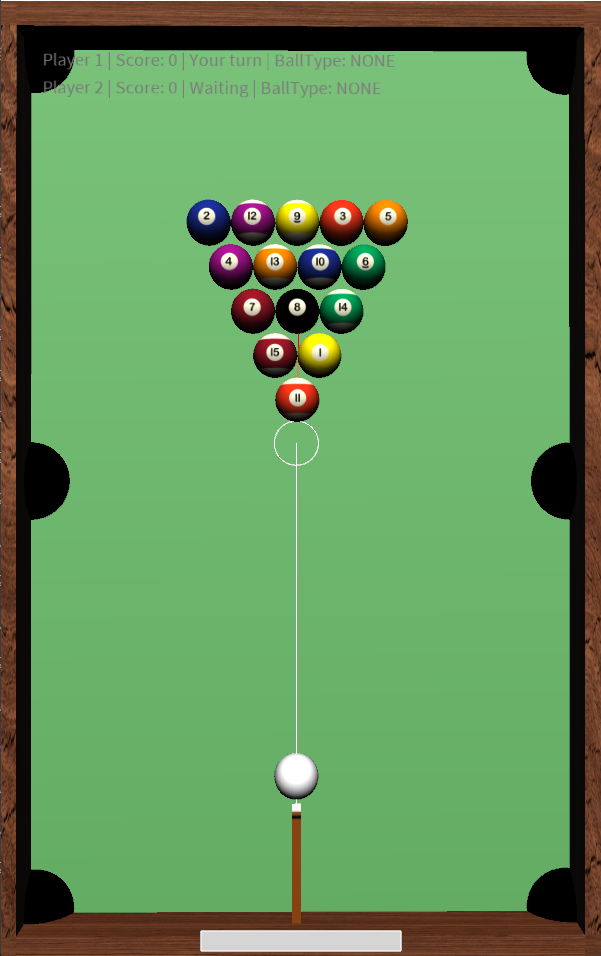
\includegraphics[width=0.5\textwidth]{../../data/Dokumentation_ScreenShots/GameAufstellung.png}
		\caption{Screenshot des Billardspiels}
	\end{figure}


	
	\subsection{Mathematische Berechnungen}
	Für die Berechnung der Kollisionen wird die Distanz zwischen den Mittelpunkten der Kugeln verwendet:
	\[
	d = \sqrt{(x_2 - x_1)^2 + (y_2 - y_1)^2}
	\]
	Wenn \( d \) kleiner ist als die Summe der Radien der Kugeln, erfolgt eine Kollision.
	
	\newpage
	
	\section{Fazit und Ausblick}
	Das Projekt hat erfolgreich ein Billardspiel simuliert, das grundlegende Physikberechnungen für die Kollisionen der Kugeln durchführt. In Zukunft könnte das System erweitert werden, um komplexere Spielmechanismen zu unterstützen und die Leistung zu optimieren.
	
\end{document}
